% WORKING DRAFT of the MARL paper (readiness audit P0.4, 28/09/2026).
% Venue template NOT chosen: the track (CCSC Eastern faculty/student or other) is unconfirmed.
% This draft uses a neutral article class with the corpus macros; switch to the venue template
% once the track is confirmed.  Every number below is copied from a named artifact.  The
% learned-actor (E3) numbers are DEVELOPMENT results; no confirmatory E3 run exists yet (28/09 self-audit:
% research/papers/audits/MARL_SELF_AUDIT_LEDGER_20260928.md).  Build: tectonic -X compile paper_marl.tex --keep-logs
\documentclass[11pt]{article}
\usepackage[margin=1in]{geometry}
\usepackage{amsmath,amssymb,amsfonts,amsthm}
\usepackage{graphicx,booktabs,url,xcolor}
\usepackage[hidelinks]{hyperref}
\usepackage{newunicodechar}
\newunicodechar{₀}{\textsubscript{0}}
\graphicspath{{../../marl_budget/figures_20260928_v4/}}

\newtheorem{theorem}{Theorem}
\newtheorem{proposition}[theorem]{Proposition}
\theoremstyle{definition}
\newtheorem{definition}[theorem]{Definition}
\newtheorem{remark}[theorem]{Remark}

\newcommand{\lean}[1]{\textsf{\footnotesize #1}}
\newcommand{\leanbox}[1]{\par\vspace{2pt}\noindent{\raggedright\footnotesize\textsf{Lean: #1}\par}\vspace{2pt}}
\newcommand{\PROVED}{\textsc{proved}}
\newcommand{\NUM}{\textsc{numerical}}
\newif\ifshownotes\shownotestrue
\definecolor{notecol}{RGB}{0,70,190}
\definecolor{todocol}{RGB}{190,20,20}
\newcommand{\NOTE}[1]{\ifshownotes{\color{notecol}\,\textsf{\footnotesize[N: #1]}}\fi}
\newcommand{\TODO}[1]{\ifshownotes{\color{todocol}\,\textsf{\footnotesize[TODO: #1]}}\fi}
\newcommand{\TODOPAR}[1]{\ifshownotes\par\vspace{2pt}\noindent%
  {\color{todocol}\textsf{\footnotesize\textbf{To decide.}\;#1}}\par\vspace{2pt}\fi}

\begin{document}
\title{Committed Priorities, Bounded Revision, and Paid Bids\\for Budgeted Multi-Agent Communication}
\author{\TODO{authors and affiliation after the track is confirmed}}
\date{Working draft, 28 September 2026}
\maketitle

\TODOPAR{Confirm venue and track (CCSC Eastern faculty or student track, page limit, anonymity) with
the advisor before any layout work. Section~\ref{sec:prelim} uses a fixed max-pressure actor;
Section~\ref{sec:e3} reports learned-actor DEVELOPMENT results only. On those, the method-scope
condition (an incremental benefit of the proposed selector under fair accounting) is NOT met; the
confirmatory run (seeds 1301--1316, after a freeze) has not been made. Whether to keep the method
framing or change the scope is the authors' decision, not the draft's.
CORRECTED 30/09 (ledger L-105, L-109, L-113 -- L-116): claim A1 (the competence margin over max pressure) and gate G1
(message use) are superseded as stated in Section~\ref{sec:e3}. A relay design is under a separately preregistered test
(PROTOCOL\_E3\_RELAY\_ROTATION\_20260930); nothing from it is in this draft.}

\begin{abstract}
When several receivers share one broadcast but can each decode a different number of messages,
a scheduler that commits to one priority before the budgets are known pays a price whenever the
joint value of messages interacts. We separate three sources of loss: the geometric cost of
commitment, which a bounded number $R$ of post-reveal revisions reduces; the cost of choosing
revisions without knowing how the actors will respond; and the cost of the byte budget
itself. The geometry is proved in Lean: a deployable regret bound with every error named, a
per-receiver block frontier, an exact non-nested team game, and a linear lower bound on the
nesting degree. Calibration of ambiguous repairs has lower and upper bounds that agree up to a
logarithmic factor on a stated Gaussian needle class. On CityFlow with a fixed max-pressure actor, a one-byte receiver
bid, charged inside the same byte cap, improves held-phase selection on fresh traffic, but its
closed-loop benefit is small. With learned MAPPO actors, no legal
selector variant improves on the committed prefix on development data, although an oracle over the
same candidates gains substantially; single- and multi-receiver loss decompositions place most of the
loss in the selectors' choice within the scored candidates, mainly the critic's ranking, with smaller but
nonzero costs of bounded revision and candidate coverage. Two later development checks change how these
actors must be read: the max-pressure reference is harmed by its own neighbour messages (a message-free
max-queue rule has about 14\% less waiting), so the learned actors' margin shrinks from 9.5--24\% to at most
6\%, and the warm-started actors lose to max-queue; and an actor co-trained without any messages (zero bytes)
has 8\% less waiting than the committed-prefix system, so the preregistered message-use gate measured
dependence on messages, not a benefit of communication. \TODO{confirmatory run after the freeze (F6); rewrite from it.}
\end{abstract}

\section{Introduction}
\begin{figure}[t]
\centering
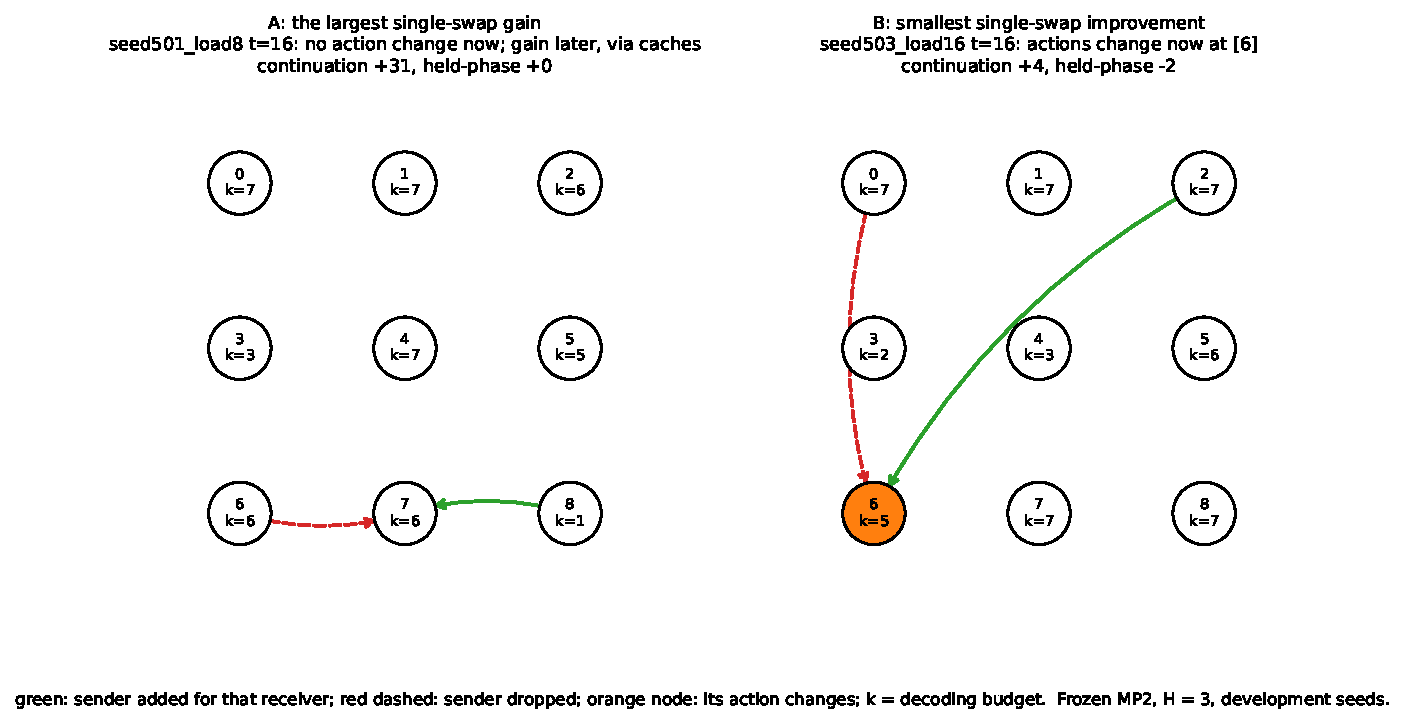
\includegraphics[width=0.9\linewidth]{fig1_scene.pdf}
\caption{Two real decision states (3$\times$3 grid, decoding budgets $k$, fixed max-pressure actor,
development seeds). A single swap for one receiver (green: sender added; red: dropped) gains 31 units
of waiting over the next three decisions although no action changes at the current step: the benefit
arrives through what the receiver caches for later decisions, which a held-phase label scores as zero.
In the right state the best single swap gains little. \NOTE{scripts/MARL\_make\_fig1\_scene.py;
target\_diag\_20260928\_000455}}
\label{fig:scene}
\end{figure}

The question we keep is: when receivers have different decoding budgets, is coordination lost
through commitment, through the limited repair budget, or because the scheduler does not know
how the actors will react; and what can a small paid bid buy back?

\paragraph{Contributions (scoped to what is established).}
\begin{enumerate}
\item A protocol for one shared broadcast with heterogeneous receiver decoding budgets, committed
  order, $R$ post-reveal revisions, explicit byte accounting and a legal/privileged information
  split (Section~\ref{sec:protocol}).
\item Revision geometry with every deployable error named (Theorem~\ref{thm:t1}), and its
  per-receiver form (Theorem~\ref{thm:block}); both machine-checked.
\item The calibration cost of ambiguous repairs on a stated class (Theorem~\ref{thm:t2}).
\item An empirical audit on CityFlow that measures oracle headroom, what legal information can
  learn, and closed-loop transfer, including the negative results (Section~\ref{sec:prelim}).
\end{enumerate}
\NOTE{Novelty is written narrowly: learned scheduling (SchedNet) and request/confidence
communication (Where2comm) already exist; one ordering for all cardinalities exists in
incremental maximisation. Our object is the interaction-dependent quantitative cost of committed
priorities and bounded revision, separated from the information needed to choose revisions.}

\section{Related work}
\paragraph{Learned communication.} Learning who talks under a shared bandwidth is established:
SchedNet learns a scheduler, encoder and actor end to end~\cite{schednet}; NDQ minimises messages
while keeping action-relevant value decompositions~\cite{ndq}; CASEC prunes coordination-graph edges
while preserving Max-Sum action choices~\cite{casec}; M2I2 selects informative state dimensions and
infers teammates' joint actions with an inverse model~\cite{m2i2}; MUTE values messages
counterfactually and preserves joint return with a conditional bound~\cite{mute}; Where2comm
requests spatially confident features in cooperative perception~\cite{where2comm}. Action relevance,
joint-action prediction and decision-preserving pruning are therefore not claimed as new here; our
object is the price of \emph{committing} one order before heterogeneous budgets are revealed, what
a bounded number of revisions buys back, and what information and calibration are needed to choose
revisions. Our SchedNet comparison is a frozen-actor adaptation (learned one-byte sender weights),
not a reproduction of the original joint training.
\paragraph{One order for all budgets.} Incremental maximisation studies one ordering good for every
cardinality with competitive ratios for monotone and submodular classes~\cite{bernstein2022,bienkowski2026}.
Dense Coverage, Sparse Refinement uses a nested top-$N$ selection of an additive surrogate within a
fused perception model~\cite{densecoverage}; our theory instead parameterises the price of nesting by
the interaction of the decision value and covers non-submodular losses.
\paragraph{Traffic.} Traffic-signal MARL on CityFlow~\cite{cityflow,colight}; max-pressure
control~\cite{varaiya2013}; dataset aggregation against covariate shift~\cite{dagger}; MAPPO with a
centralised critic~\cite{mappo}.

\section{Problem, protocol and information}\label{sec:protocol}
Senders and receivers are the $m$ intersections. At every decision step:
(1) the public context $z$ holds the payloads paid in earlier steps and the time;
(2) the scheduler commits a base order $\pi$ before the capacity vector $K$ is known;
(3) $K$ is revealed, $k_i$ being the number of other payloads receiver $i$ decodes;
(4) each receiver gets a set $S_i$ with $|S_i|=k_i$ exactly, and $|S_i\setminus P_i|\le R$, where $P_i$ is
the first $k_i$ entries of $\pi$ without $i$;
(5) the union is broadcast once, each receiver decodes exactly $S_i$, and the actors act.

\paragraph{Bytes.} A profile is charged the cheaper of its patched description
($25|T| + 3\cdot\#\text{replacements}$, with $T$ the stream prefix plus patches) and its explicit
description ($25|\bigcup_i S_i| + 2$ bytes per receiver). Explicit profiles are therefore allowed:
capacity is a \emph{decoding} budget, not a listening-time prefix, and nesting is not forced
inside the policy class. $R=0$ is the committed-order model and direct (unrestricted) selection is
a legitimate comparator that measures the price of commitment. Receiver bids are charged inside
the same total cap at every step. Delivery delay is zero.
\NOTE{PROTOCOL\_HETERO\_v0.md and its Amendment 1.}

\paragraph{Information.} Legal scheduler information is the paid cache $z$, a receiver mirror of
every receiver's cache (asserted equal after every transmission), the public topology and the
known actor code. Privileged quantities (fresh states, counterfactual actions, oracle rollouts)
may generate labels or diagnostics only; every deployable run is wrapped so that any oracle call
fails, and closed-loop reports check the access log.

\section{Methodology}
The same protocol is run with two actors; the selector recipe differs only where the actor does.
\paragraph{Receiver bid (both).} Before transmission each receiver computes, from its own view, its
actor's best and runner-up phases and a 2-bit gap bin (1 byte, plus a 1-byte header), charged inside
the total cap at every step.
\paragraph{Candidates and policies (both).} The candidate family is every one-swap plus random
profiles with radius $\le 1$, $\le 2$ and unrestricted; ``R1'' restricts the output to radius 1 and
``direct'' does not. Exact enumeration of $F_R$ is infeasible at $m=9$ receivers and is not claimed.
Scores are anchored to the prefix; a threshold $\tau$ chosen on a select split decides whether to
edit. For the closed-loop selectors the grid is $\{-\infty, 0\}$ plus two score quantiles, with no
``always keep the prefix'' option; the development diagnostics of Section~\ref{sec:e3} add
$\tau=+\infty$.
\paragraph{Recipe M (fixed max-pressure actor).} Target: the held-phase value (the joint action of a
profile held for $H=3$ decisions). A stage-A model predicts, per candidate and receiver, whether the
actor plays the first or second phase of its bid or another (three classes), trained on privileged
counterfactual actions as training labels only; a critic scores candidates from $z$, $K$, the bid and
the predicted soft joint action.
\paragraph{Recipe L (learned actor).} The actor is trained by MAPPO with a centralised critic on the
team reward, from scratch or warm-started by behaviour cloning of max pressure on the same restricted
views (Section~\ref{sec:e3}). Target: a declared continuation value
$f^{\pi,c}_X(S)$ --- profile $S$ at the current step, then three decisions of the committed prefix
with the same frozen actor --- because the held-phase target captures only about half of the
continuation headroom (Section~\ref{sec:prelim}). A binary response head predicts, per candidate and
receiver, whether the actor's current action changes from its action under the prefix, trained on the
actor's stored joint actions (training labels only); the critic receives the predicted change
probabilities. Variants: no bid, bid, head without bid, bid and head; a same-byte queue bid as the
alternative-information control.
\section{Theory}\label{sec:theory}
Let $f$ be any set function (the team decision value of a broadcast set, fixed controller,
fixed state), $w$ any score, and $\mathrm{ScoreLocal}(f,w,\eta)$ the hypothesis that every
marginal $f(A\cup\{i\})-f(A)$ is within $\eta$ of $w_i$.

\begin{theorem}[Deployable regret, \PROVED]\label{thm:t1}
Suppose the true local interaction is $\delta$ and the score is within $u$ of the true first-order
gains, $P$ is top-$k$ by the score, the selector returns $\hat S$ in a candidate family $C$ with
$\hat f(\hat S)\ge \hat f(S')-\nu$ on $C$, $|\hat f-f|\le\varepsilon$ on $C$, and every set reachable
with $R$ replacements is within $\zeta$ of some candidate. Then for every $k$-set $T$,
\[ f(T)-f(\hat S)\;\le\;2(\delta+u)\,(|P\setminus T|-R)_+ + 2\varepsilon+\nu+\zeta. \]
The coefficients of $u$ and $\varepsilon$ are attained.
\end{theorem}
\leanbox{LeanMarlEstimatedRevisionV1.deployed\_regret, score\_error\_sharp, eval\_error\_sharp,
hypotheses\_satisfiable (gate smokeMARL17\_20260927)}

\begin{theorem}[Per-receiver block frontier, \PROVED]\label{thm:block}
Encode a profile as a set of receiver--sender edges with receiver blocks. If
$\mathrm{ScoreLocal}(f,w,\eta)$ holds and $P$ is top-$k_b$ by $w$ inside every block, then for
every block-feasible $T$ some block-feasible $S$ with at most $R$ replacements per block has
$f(T)-f(S)\le 2\eta\sum_b(|P_b\setminus T_b|-R)_+$; a per-block cut margin $2\eta$ makes the
prefix optimal.
\end{theorem}
\leanbox{LeanMarlBlockFrontierV1.block\_frontier, block\_zero\_price,
block\_hypotheses\_satisfiable (gate smokeMARL4\_20260927)}

\begin{remark}[Where the deployed loss goes]
For a fixed value $f$ and nonempty families $F_{\rm all}\supseteq F_R\supseteq F_{R,B}\supseteq C$
(all profiles; radius $R$; radius $R$ and byte cost $\le B$; the scored candidates), with
$V_D=\max_{S\in D}f(S)$ and output $\hat S\in C$,
\[ V_{\rm all}-f(\hat S) = (V_{\rm all}-V_R) + (V_R-V_{R,B}) + (V_{R,B}-V_C) + (V_C-f(\hat S)), \]
the commitment (geometric) loss, the byte-feasibility loss, the candidate-coverage loss and the
estimation/search loss. The last term is at most $2\varepsilon+\nu$ (the argument of
Theorem~\ref{thm:t1}). The first is bounded by Theorem~\ref{thm:block} only when its hypotheses
hold; the runtime order in our experiments is a cached-queue order, not a top-score order of the
same vector, so we do not assume that bound in traffic; Section~\ref{sec:e3} measures every term
on a reduced, fully enumerated panel. A bid of $B_{\rm bid}$ bytes leaves
$B-B_{\rm bid}$ for payloads and adds information: a trade-off, not a theorem that bids help.
\end{remark}
\NOTE{This identity is telescoping algebra; the $2\varepsilon+\nu$ part is \lean{deployed\_regret}.
Not a new Lean module.}

\begin{theorem}[Calibration of ambiguous repairs, \PROVED]\label{thm:t2}
On the needle class over one Gaussian query channel (known first-order gains, interaction $\beta$
on one unknown reachable set), every protocol acceptable with probability $1-\alpha$ spends at
least $|\mathrm{Amb}|\,((1-\alpha)\log(1/\alpha)-\log 2)/(\beta^2/2)$ expected rollouts at the null
world, and a protocol that never queries some ambiguous repair cannot be acceptable. If every
reachable $T\ne P$ has first-order deficit above $\varepsilon$, block tests with
$\lceil 8\log(|\mathrm{Amb}|/\alpha)/\beta^2\rceil$ rollouts per ambiguous repair are acceptable at every
world of the class.
\end{theorem}
\leanbox{LeanMarlRepairCalibrationV1.calibration\_lower, zero\_allocation\_impossible,
calibration\_upper (gate smokeMARL17\_20260927); fixed schedules: LeanMarlCalibrationGapV1;
shared pairs: LeanMarlPairCalibrationV1 (gate smokeMARL4\_20260927)}

\paragraph{Scores that do not know the interaction.} On the executable E1b task the mean value is
edge-local with scores $g_i^2$ and constant $\beta^2$; the uniform score $g_i^2+\beta^2/2$ for \emph{every}
message halves the constant without knowing which pair interacts, and preserves every ranking \PROVED.
\leanbox{LeanMarlE1bUniformV1.e1b\_scoreLocal\_uniform, uniform\_shift\_order, e1b\_uniform\_satisfiable (gate smokeE1bU\_20260928)}

\paragraph{Also proved.} Zero price under a $2\delta$ cut margin with a sharp constant
(\lean{LeanMarlSubsetFrontierV1}); an exact non-nested three-message team game with randomised
price $p(1-2p)$ closed by one revision (\lean{LeanMarlXorGameV1}); the nesting degree is at least
$\lfloor (m+1)/4\rfloor$ (\lean{LeanMarlNestingDegreeGeneralV1}); equality is a conjecture supported
by exhaustive search for $m\le 8$.

\section{Experimental design}
\paragraph{Controlled calibration (E1).} E1a is the exact T2 needle model; E1b is an executable
Bayes-decoder task with a hidden interacting pair, which is \emph{not} the Gaussian channel of
Theorem~\ref{thm:t2}. \NOTE{E1\_CONTROLLED\_RESULTS\_20260927.md; targeted $\equiv$ uniform is a
negative control.}
\paragraph{Traffic.} CityFlow $3\times3$ grid, two headways, i.i.d.\ capacities
$k_i\sim U\{1,\dots,7\}$, cap $+84$ bytes over the prefix bytes. Splits by traffic seed: train
301--364, select 401--408, development 501--508, fresh confirmation panels 601--616 (B2/B3),
801--816 (B4), 1101--1116 (descriptive). Endpoints: sum of waiting (primary), finished and
unfinished trips, throughput, censored travel time, total bytes. Paired by episode; bootstrap over
episodes; selector init seeds averaged per episode.
\paragraph{Learned actors (E3).} Protocols are written before results: actor seeds per recipe; gates G1
(the actor uses messages: removing them changes at least 10\% of actions and worsens closed-loop
waiting) and G2 (within 10\% of max pressure on the select split); the warm-started recipe is gated
on its pilot seed, the scratch recipe per seed, and every actor outcome is reported. \emph{Correction:} G1
tests whether an actor's decisions depend on its messages, not whether communication helps, and G2 was
calibrated against a max-pressure reference that its own message use harms (Section~\ref{sec:e3}). Both gates
are kept as recorded; neither is read as evidence of communication value. The benefit comparators are a
same-recipe actor trained without messages and the message-free max-queue rule. Selector labels
and tuning use train/select/development seeds only; closed-loop development uses a pilot panel
(901--916); seeds 1301--1316 are reserved for one frozen confirmatory run. Comparators on the SAME
frozen actor: committed prefix, direct selector without bid, response-bid selector, R1, learned
SchedNet-style adaptation, same-byte queue bid, and an oracle diagnostic. Costs: total charged bytes
(payload, control, bid) and compute; frontier at caps $+28$, $+56$, $+84$, $+140$.
\TODO{final protocol and freeze manifest (handoff F6) before the confirmatory run.}

\section{Preliminary results on a fixed max-pressure actor}\label{sec:prelim}
\NOTE{Every number here uses the frozen MP2 actor. None is the learned-MARL headline.}

\paragraph{Oracle headroom.} With the exact oracle over $F_R$, $R=1$ recovers 88\% of the gap to
private unrestricted sets on 16/16 episodes \NUM.
\NOTE{HETERO\_EXACT\_RESULTS\_20260927.md}

\paragraph{Held phase, preregistered (B2).} On fresh seeds 601--616, the frozen response-bid
direct selector beats the better no-bid learned control by $+1.85$ $[+0.95,+2.84]$, about 18\% of
the oracle gain \NUM. \NOTE{B2\_CONFIRMATION\_RESULTS\_20260927.md}

\paragraph{Closed loop, preregistered (B3, B4).} The frozen models give no closed-loop benefit
(B3: $-0.26\%$ $[-1.20,+0.62]$ against the control) and edit in about 2 of 26 steps per episode (range 1--5), against 19 for the oracle. After one
DAgger iteration (B4, fresh seeds 801--816) the registered comparison passes: $-1.49\%$
$[-2.75,-0.23]$ in waiting against the retrained control. Against the prefix the change is
$-0.68\%$ $[-2.87,+1.37]$, no better than the frozen design, while the held-phase oracle reaches
$-15.0\%$ (Figure~\ref{fig:b4}) \NUM.
\NOTE{B3\_CLOSED\_LOOP\_RESULTS\_20260927.md, B4\_DAGGER\_RESULTS\_20260928.md}

\begin{figure}[t]
\centering
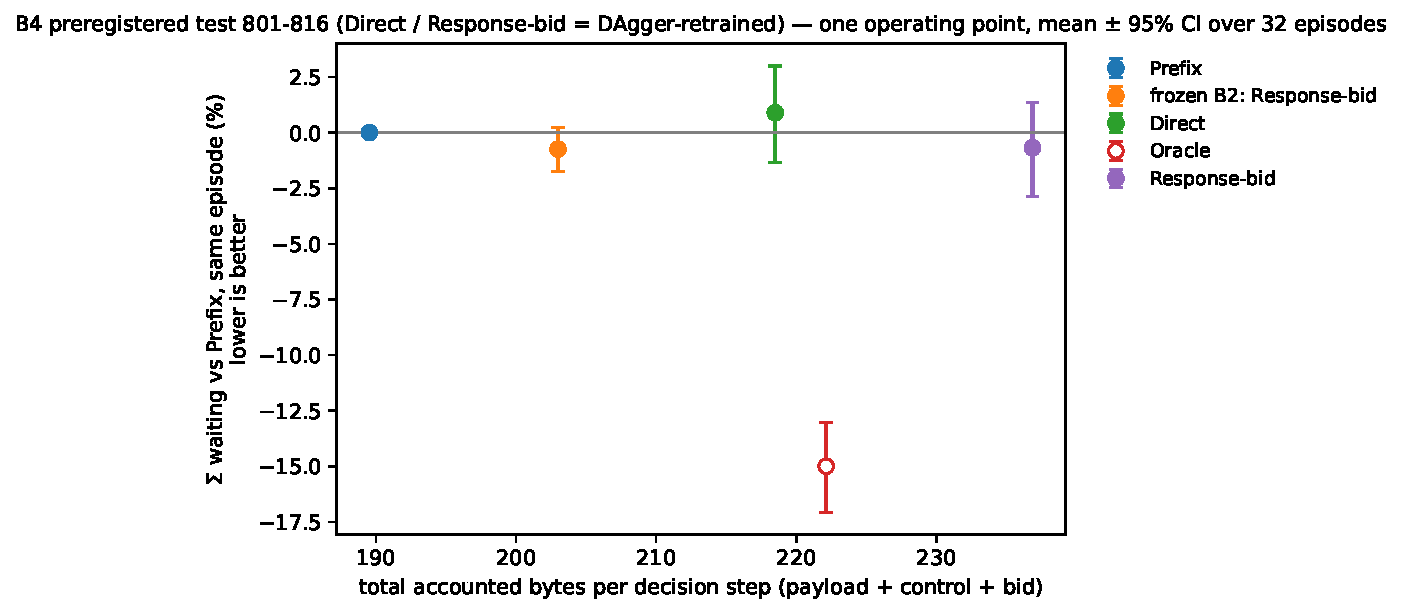
\includegraphics[width=\linewidth]{fig3v4_b4test.pdf}
\caption{Closed loop on the preregistered B4 panel (32 episodes, frozen MP2 actor, one operating
point, lower is better). Direct and Response-bid are the DAgger-retrained selectors; hollow:
held-phase oracle reference. \NOTE{caption file fig3v4\_b4test.caption.txt}}
\label{fig:b4}
\end{figure}

\begin{figure}[t]
\centering
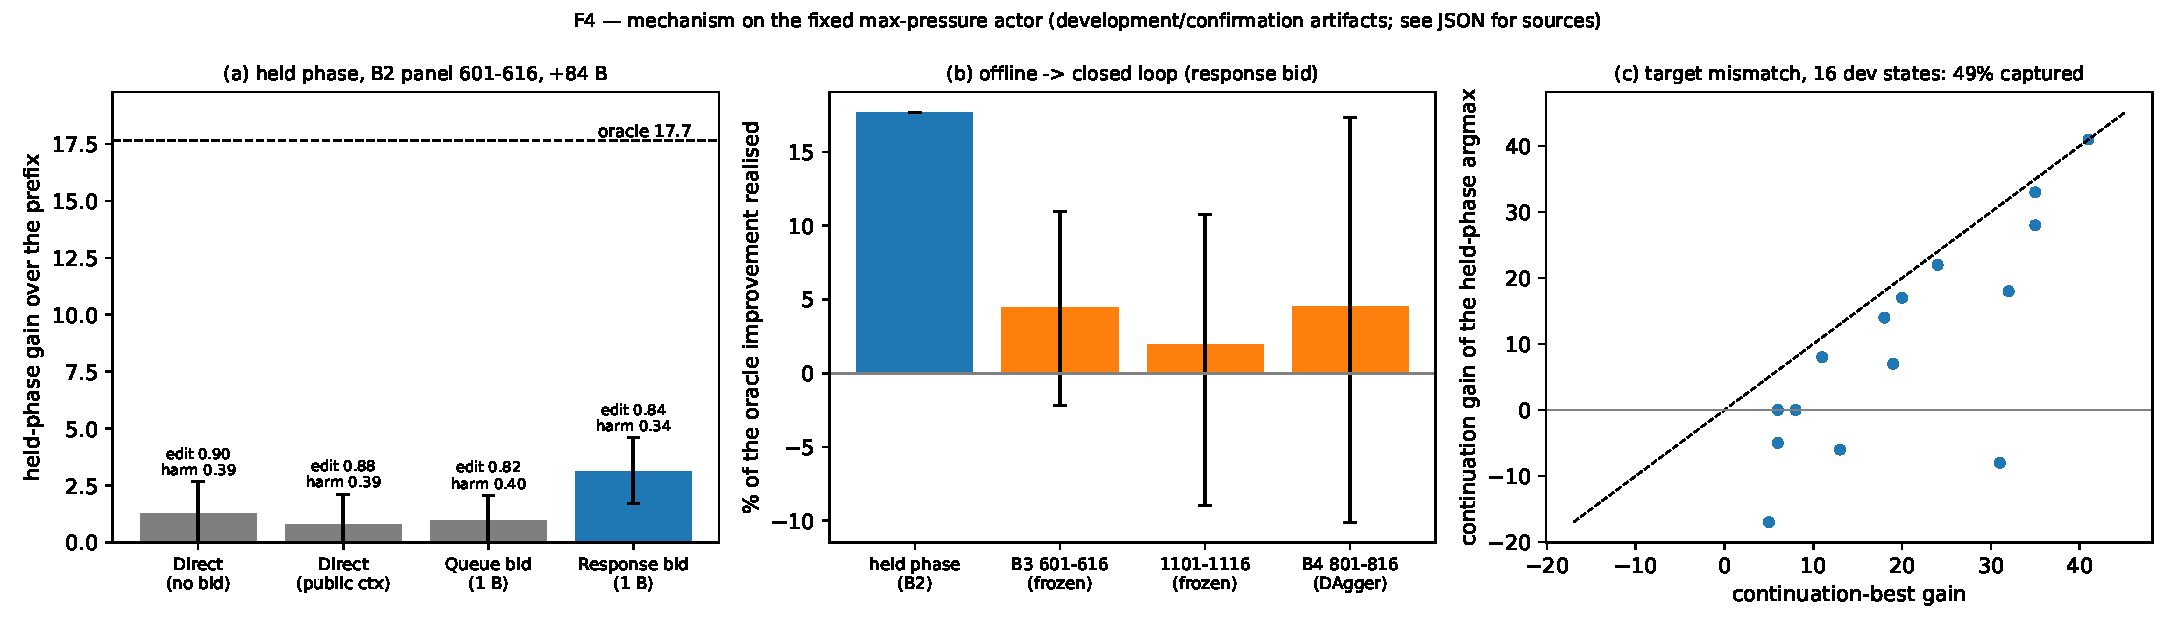
\includegraphics[width=\linewidth]{fig4_mechanism_mp2.pdf}
\caption{Mechanism on the fixed max-pressure actor. (a) Held-phase gain on the preregistered B2 panel
(+84 bytes, direct), with edit rate and the share of edits that harm; dashed: oracle over the same
candidates. (b) Share of the oracle's improvement realised by the response-bid selector, held phase
against three closed-loop panels (95\% episode bootstrap). (c) Continuation gain of the held-phase
argmax against the continuation-best gain on 16 development states; the dashed line is no mismatch.
\NOTE{producer scripts/MARL\_make\_fig4\_mechanism.py; numbers in fig4\_mechanism\_mp2.json}}
\label{fig:mech}
\end{figure}

\paragraph{Target mismatch.} On 16 development states, the held-phase argmax coincides with the
continuation argmax in 1 state, captures 49\% of the one-step continuation headroom and is worse
than the prefix in 4 states \NUM. The held-phase target therefore caps what a perfect learner of
that label can achieve, while estimation error remains the larger factor.
\NOTE{TARGET\_DIAG\_RESULTS\_20260928.md}

\paragraph{Comparators.} An independently tuned direct selector does not change the $+84$
operating point, and bounded repair (R1) is below it at $+56$ and $+84$ bytes on development data,
so we make no claim that bounded repair beats direct selection. Two heuristic communication
baselines (a fresh-queue sender weight and a request rule on the same bid) give no closed-loop
benefit. \NOTE{BASELINES\_DIRECT\_STAGEA2\_RESULTS\_20260927.md; heuristics, not learned SchedNet or
Where2comm.}

\paragraph{Latency.} Post-grant scheduler compute for the response-bid selector: median 14.8 ms,
p95 16.1 ms on an idle CPU; the prefix takes 0.007 ms. No uplink or network delay is modelled, so
this is not an end-to-end deadline claim. \NOTE{latency\_b2\_idle\_20260928\_000900}

\section{Results with a learned actor}\label{sec:e3}
\NOTE{Development evidence only: labels and message use on split 501--508, closed loop on the pilot
panel 901--916, both opened. Protocols PROTOCOL\_E3\_PILOT, \_SCRATCH, \_ABLATION (Amendment 1),
\_DELAY\_ACQ and \_MIXACTOR were written before their results. Actor seeds 3 and 4 of both recipes
were launched before any E3 result but are not in the protocols' seed lists (declared:
MARL\_SELF\_AUDIT\_LEDGER\_20260928.md, L-25). Seeds 1301--1316 are untouched. Sources:
E3\_INTERIM\_RESULTS\_20260928.md.}

\begin{figure}[t]
\centering
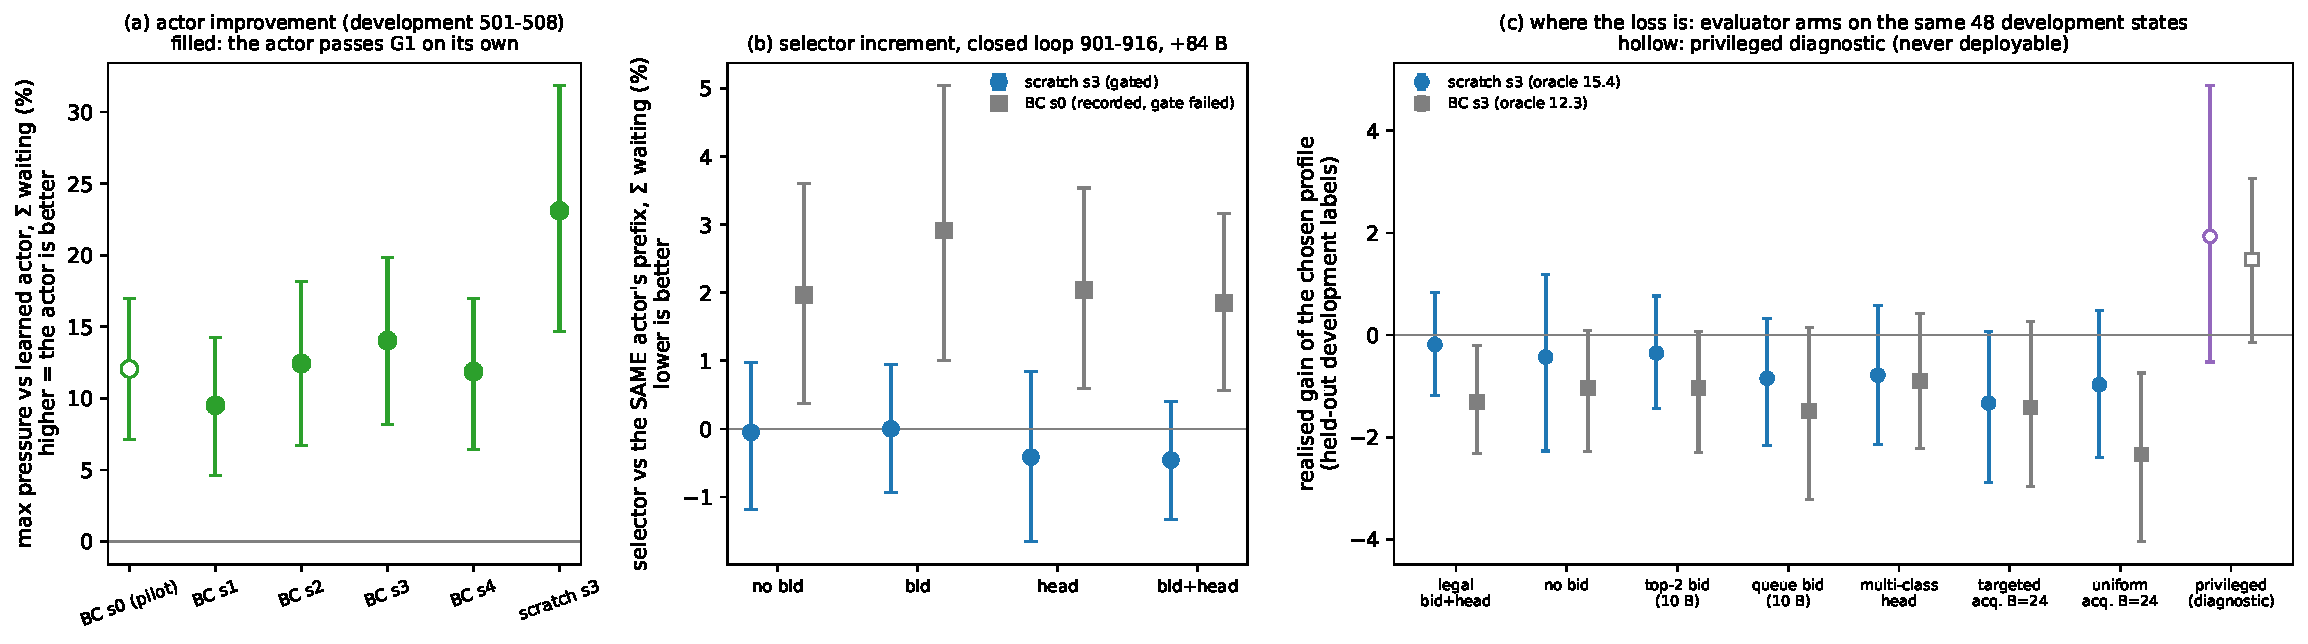
\includegraphics[width=\linewidth]{fig_e3.pdf}
\caption{Learned actors, development data. (a) Actor improvement: max pressure's extra total waiting
against each finished learned actor with the same communication; this reference is harmed by its own
message use, see the correction in the text (filled: the actor passes the
message-use gate G1 on its own; the warm-started recipe is gated on its pilot seed s0, which fails).
(b) Selector increment on the SAME actor: each variant against that actor's committed prefix, closed
loop, +84 bytes, three init seeds averaged per episode (grey: the warm-started pilot actor, recorded
under its failed gate). (c) Realised gain of the profile each evaluator chooses on the same 48 held-out
development states of two actors; hollow: an evaluator told the actor's actual joint actions
(privileged, diagnostic only). The oracle over the same candidates gains $+15.4$ and $+12.3$. All
intervals: 95\% bootstrap over episodes. \NOTE{scripts/MARL\_make\_fig\_e3.py; numbers in
fig\_e3.json; panel (c) from MARL\_e3\_paired\_eval.py (e3\_dev\_arms.json).}}
\label{fig:e3}
\end{figure}

\paragraph{Actor.} Each receiver's actor reads only its own view through an adapter that encodes, per
other agent, whether a message is fresh, whether the agent was ever heard, the message age, the
payload and static public topology; a missing message is distinct from a zero payload. It is
trained by MAPPO on the team reward with a centralised critic that sees a privileged global state
during training only; one recipe warm-starts it by behaviour cloning of max pressure on the same
restricted views, the other trains from scratch.

\paragraph{Competence and message use.} Eleven actors have finished: the warm-started recipe with seeds
0--4, the from-scratch recipe with seeds 0--4, and one mixed-profile pilot (below). With the same
communication, max pressure as implemented has 9.5\% to 24\% more total waiting than each of them, every
95\% interval above zero (Figure~\ref{fig:e3}a) \NUM. That reference is weak. On the 128-episode development
panel (traffic seeds 901--964, headways 8 and 16\,s), the same rule without its downstream, message-fed
terms, a max-queue controller that uses no messages, has about 14\% less waiting than max pressure with the
prefix deliveries, and still 13\% less with full delivery; pressure variants on vehicle counts are worse, not
better. Against max-queue, the five warm-started actors are \emph{worse} ($+1.2\%$ to $+5.5\%$, every
interval above zero) and the five from-scratch actors only $1.7\%$ to $6.3\%$ better \NUM. Competence is
therefore stated against max-queue, not max pressure. \NOTE{L-114 -- L-116; e3\_mp2\_message\_check\_20260929,
e3\_mp2\_message\_check\_v2\_20260929.} All five from-scratch actors pass both gates: removing all
messages from the input costs them $+4.3\%$ to $+8.7\%$, every interval above zero also when clustered
by traffic seed, and scrambling sender identities costs $+3.1\%$ to $+11.6\%$.
In the warm-started recipe message use varies by seed: $+0.4\%$ (not significant) for the pilot seed
and $+3.0\%$ to $+17.5\%$ for the other four. The pilot seed therefore fails the preregistered gate G1,
and that recipe's selector results are recorded, not read as a method result. Actors trained on at most
seven decoded messages degrade when all eight are delivered, an instance of the train/deploy shift that
makes ``more information'' not automatically better for a fixed actor.

\paragraph{Passing G1 does not show a benefit.} On the same 128-episode panel, an actor trained with the
from-scratch recipe but without any messages (zero bytes) has $8.0\%$ $[7.4, 8.6]$ less waiting than the
committed-prefix system of the five from-scratch actors, and less than each of them ($5.6\%$ to $10.5\%$); a
second training seed gives $7.9\%$. Doubling the prefix actor's training to 4000 iterations leaves it $6.3\%$
$[5.3, 7.4]$ worse than the no-communication actor trained for the same number of iterations \NUM. Under this
protocol's capacity process, learning from the prefix's partial, priority-biased messages harms these flat
actors, so every selector result below is measured on top of actors that ignoring communication would beat.
\NOTE{L-105, L-109, L-113; e3\_codesign\_eval\_20260929. Development panel, two no-communication seeds.}

\paragraph{Mixed-profile actor (pilot, one seed).} To separate the scheduler from an actor adapted to
the prefix, one actor was trained from scratch with half of its training steps on random feasible
profiles within the same cap (checkpoint selection under the prefix). It is as competent as the
prefix-trained actors (max pressure $+22.4\%$), but it fails the closed-loop part of G1: removing all
messages from its input changes 43\% of its actions yet total waiting by only $-0.9\%$ $[-2.3,+0.6]$
(traffic-seed clusters). Old messages hurt it clearly ($+7.5\%$ $[+5.7,+9.5]$), and so do scrambled
identities ($+4.9\%$); full delivery changes waiting by $-1.9\%$, not significant. Against the
prefix-trained seed-3 actor on the same episodes its waiting differs by $+0.6\%$ $[-1.8,+3.1]$, neither
an advantage nor a shown equivalence \NUM. The ``no message'' variant removes messages from the actor's
input only (the prefix is still sent), so it is not a zero-byte deployment. Its selector results are
pending and, after the G1 failure, diagnostic only.
\NOTE{e3\_mixactor\_20260928/actor\_s3; PROTOCOL\_E3\_MIXACTOR\_20260928.md; one seed supports a
robustness observation, not a causal claim about mixture training.}

\paragraph{Delayed observations (stress test).} When every receiver acts on the messages it held $d$
decisions earlier (ages increased; scheduler, mirror and bytes unchanged), the from-scratch actor loses
$+3.9\%$ $[+1.8,+6.2]$ at 20\,s and $+5.6\%$ $[+3.3,+8.3]$ at 30\,s, the warm-started seed-3 actor is
insensitive, and max pressure \emph{improves} by 3--7\%, as expected from its harmful use of messages
above. Max pressure's excess over the from-scratch actor
shrinks from $+24\%$ to $+9.5\%$ $[+5.8,+13.1]$ at 30\,s but stays positive \NUM. This delays the
receivers' observations under an idealised scheduler; it is not a network-delay test of the
bid--select--transmit loop. \NOTE{e3\_delay\_v2\_20260928, pilot panel, 32 episodes; the $d=0$ encoding
and max-pressure identities and a causality assertion on payload times hold.}

\paragraph{Learned scheduling baseline.} A SchedNet-style scheduler that learns each sender's one-byte
weight from its own sensor by policy gradient on the team reward does not beat the committed
cached-queue priority with the same actor. For the gated from-scratch actor and the warm-started seed-3
actor, with three init seeds each, the learned schedule changes total waiting by $+0.4\%$ to $+4.8\%$
(worse in every run, significantly so in two of six) \NUM. \NOTE{e3\_schednet\_v2\_20260928; weights
quantised to one byte before the stream is ordered; trained on float scores.}

\paragraph{Selection on top of a learned actor.} We ported the selector of Section~\ref{sec:prelim} to
the learned actor with a declared-continuation target and four variants: no bid, the one-byte bid (the
actor's own top-two actions and logit gap), a response head without the bid, and bid plus head. For
the from-scratch actor that passes both gates, no variant changes closed-loop waiting against the
committed prefix (bid plus head $-0.46\%$ $[-1.33,+0.41]$; the others within $\pm0.5\%$;
Figure~\ref{fig:e3}b), although an oracle over the same candidates gains $+15.4$ units per state on
held-out labels \NUM. For the warm-started actors (recorded under their recipe's failed gate) every variant is worse than the
prefix at $+84$ bytes: 1.8--2.9\% for the pilot seed and 2.5--4.1\% for seed 1, and at caps of $+56$ bytes and more the warm-started
actors' selectors are up to 4\% worse. The bid does carry response information (the head's recall of
action changes rises from 0.006 to 0.15 with it), but the critic cannot order candidates within a
state: on candidate pairs whose true gains differ it orders about half correctly (0.48--0.52, ties
counted as half; at chance, and below the 0.53 of the rule ``fewer edits first''), although it orders
65\% correctly on its own training states; its tie-aware rank correlation with the true gains is between $-0.04$ and $+0.04$, and 43--75\% of its
edits harm; the 90\% quantile of its gain error ($\approx 13$, a diagnostic, not a certified bound) is
of the order of the gains themselves \NUM. \NOTE{Pair accuracy recomputed with tie-half credit (MARL\_e3\_selector\_diag\_v3.py, MARL\_e3\_ranking\_diag\_v2.py); an earlier strict count, 0.40--0.48, scored predicted ties as wrong and is withdrawn.} Editing on such scores is editing on noise: an argmax of an
estimate with per-value error $\varepsilon$ can lose $2\varepsilon$ against the prefix, the rule ``edit
only if the estimated gain exceeds $2\varepsilon$'' never loses, and every smaller threshold, including
positive ones, can harm \PROVED; no valid bound $\varepsilon$ is available for the learned critic, so
the rule is not instantiated here.
\leanbox{LeanMarlSafeEditV1.argmax\_harm\_le, argmax\_harm\_sharp, safe\_rule\_never\_harms,
threshold\_sharp, threshold\_sharp\_positive (gate smokeSafeEdit2\_20260928)}
\NOTE{e3\_selector\_diag\_v2\_scratch\_s3.json (tie-aware; edits counted by chosen index).}

\paragraph{Where the loss is.} Figure~\ref{fig:e3}c compares evaluators on the same 48 development
states of two actors (the gated from-scratch actor and the warm-started seed-3 actor). No legal
evaluator realises a positive gain. The bid-plus-head evaluator gives $-0.19$ $[-1.18,+0.84]$ and
$-1.31$ $[-2.32,-0.20]$. Its alternatives all lie between $-2.3$ and $-0.3$ \NUM:
\begin{itemize}
\item no bid;
\item a same-byte (10-byte) queue bid instead of the response bid;
\item a multi-class head that predicts the actor's phase distribution;
\item training on 24 labels per state, chosen near bid ties or uniformly.
\end{itemize}
Of the 21 pairwise differences between legal arms per actor, one is significant (on the warm-started
actor, uniform labelling is 1.4 worse than the multi-class head). The response bid minus the queue bid
is $+0.49$ and $+0.45$, and the multi-class minus the binary head is $-0.60$ and $+0.41$. An evaluator that is
told the actor's actual joint action under every candidate (privileged, diagnostic only) realises
$+1.9$ and $+1.5$. That is better than the legal evaluator by $+2.1$ $[+0.1,+4.5]$ and $+2.8$
$[+1.0,+4.7]$; clustered by traffic seed the intervals are $[-0.2,+4.6]$ and $[+1.1,+4.7]$. Yet it is
still only about 12\% of the oracle's gain over the same candidates. Response information is therefore
part of the bottleneck, the legal predictors we tried do not recover it, and even perfect response
information leaves most of the headroom unused.
\NOTE{selectors\_v3 (privileged), v4 (same byte), v5 (multi-class head), acquisition\_v2 (legal
2-bit bins, B = 24 on every training state); f2b\_paired\_dev.json and e3\_dev\_arms.json per actor.}

\paragraph{Bridge to the theory (reduced panel).} To test whether Theorem~\ref{thm:t1} explains the
traffic object, we took 16 development states per actor and one receiver per state (the smallest bid
gap). Every other receiver keeps its prefix, and we evaluated the continuation value $f$ of all 256
sets the receiver could decode. On this whole space two linear programs give two constants: the
smallest ScoreLocal constant $\eta^\star$, and the smallest constant $\eta_{\rm top}$ under which the
deployed prefix is also top-$k$ by the same score, i.e.\ both hypotheses of the theorem at one $w$.
\begin{itemize}
\item At the smallest constant $\eta^\star$ the prefix is also top-$k$ in 5 of 16 states per actor; at
  $\eta_{\rm top}$ every state (16 of 16) has a valid instance of both hypotheses. The scores are fitted
  after the whole value table is seen, so this is a numerical instantiation on reduced objects, not a
  deployable certificate.
\item $\eta_{\rm top}$ has median 7.0 and 6.0, about the spread of $f$ over the $k$-sets (9.6 and
  8.5): first-order scores explain these values poorly.
\item The optimum is within one revision of the prefix in 15 and 13 of 16 states. The geometric loss
  at $R=1$ therefore averages 0.3 and 0.8, the $+84$-byte cap never binds, and the scored candidate
  family contains the global optimum in 15 and 13 states.
\item The valid instance of the theorem, $2\eta_{\rm top}(d-R)_+$, holds in every state (checked). It
  is zero wherever the optimum is one revision away, and 2.8 to 6.7 times the realised loss in the four
  states where it is not \NUM.
\end{itemize}
On these single-receiver objects, commitment geometry and bytes cost little and are correctly bounded,
which is consistent with an estimation bottleneck; it does not show that a selector editing several
receivers at once loses only through estimation (next paragraph).
\NOTE{scripts/MARL\_e3\_bridge\_panel\_v2.py; e3\_bridge\_v2\_\{scratch,bc\}\_s3\_20260928 (f.json holds every
value). The earlier v1 panel omitted the empty and full sets and read hTop at one LP minimiser; its
``hTop false in 16/16'' is withdrawn (self-audit L-01..L-04, L-34).}

\paragraph{All receivers at once (development panel).} The reduced panel varies one receiver; a
selector edits several. On the 48 development states of each actor we therefore decomposed the loss
on the actual multi-receiver objects. The stored labels score a candidate family whose best member
edits about six receivers. We extended it by a rollout local search over single sender swaps at any
receiver within the cap, started from the family's best profile and, separately, from the prefix.
This search is a diagnostic: it uses the simulator. The best profile found is the better of the two
searches in each state; it gains $+20.8$ and $+16.3$ over the prefix. Measured from that profile the
losses are \NUM:
\begin{itemize}
\item outside the scored family, at least $+5.3$ and $+4.0$ (a lower bound, since the search is local);
\item the radius-one restriction inside the family, $+2.7$ and $+2.5$ (inside the family only, not the
  price of bounded revision over all profiles);
\item the byte cap, about $0.1$;
\item the legal selector's choice inside its own feasible family, $+15.6$ and $+13.6$, the largest term
  by far.
\end{itemize}
The last term is not $2\varepsilon$ alone. It splits into the critic's ranking loss (the family best
minus the critic's argmax), $+15.2$ and $+14.2$, and the signed effect of the edit threshold (the argmax
minus the thresholded choice), $+0.4$ and $-0.5$, neither significant. The threshold changes 69\% and
24\% of the choices, so the deployed rule's search term $\nu$ is not zero either. Removing the threshold
does not rescue the selector: the critic's argmax realises at most $+0.44$ for any checkpoint \NUM.
A local search from the prefix alone reaches 85\% of the best found on both actors, with about 2.5 single
swaps on 2.5 receivers. The gain of a multi-receiver edit exceeds the sum of its single-receiver parts in
22 of 40 and 19 of 38 states, and falls below it in 15 and 12. On the tested objects the legal rules
therefore fail to extract headroom that a few swaps would capture, and the loss is mostly the critic's
ranking. Commitment geometry and candidate coverage are smaller but not zero once all receivers move,
and receivers interact. This does not prove that all global regret is estimation: coverage is only
bounded from below.
\NOTE{scripts/MARL\_e3\_multireceiver\_decomp.py; MARL\_e3\_mrdecomp\_report\_v2.py, whose source was lost to an overwrite and
whose outputs MARL\_e3\_mrdecomp\_report\_v3.py reproduces exactly (best found = max of both
searches per state; ranking loss and threshold effect recomputed from the checkpoints on the saved labels, choices
equal to the trainers' dev\_chosen); e3\_mrdecomp\_20260928/report\_v2.json. 48 of 48 states for both actors; one
shard reran after a CityFlow deadlock. report.json (v1) is kept.}

\paragraph{Reading.} On development data the method-scope condition is not met. No legal selector
variant improves on the committed prefix of a learned actor, in closed loop or offline. Every grounded
adaptation we registered left the realised gain at or below zero: response information, a multi-class
response head, a same-byte alternative bid and decision-targeted labelling. The dense-label round, the
from-scratch actors of other seeds and the mixed-profile actor are still running, and none of them is a
confirmatory test either.
\TODO{dense-label result (F1); scratch seeds 0, 1, 2, 4; mixed-profile actor (F2-C); frontier and shift for the from-scratch actors.}

\section{Limitations}
\begin{itemize}
\item Superseded claims: the competence margin over max pressure and gate G1 do not show that the learned
actors are competent communicators. Max pressure as implemented is harmed by its own messages, and a
co-trained actor without messages beats every prefix-trained actor on development data. Every selector result
concerns actors that ignoring communication would beat.
\item Scope of the positive results: the paid bid helps selection on the fixed max-pressure actor in
the held phase (preregistered) and only marginally in closed loop. On learned actors no selector
variant has improved on the committed prefix; this is development evidence from two actors offline and
one gated actor in closed loop.
\item Seeds: five gated from-scratch actors, but selector results so far for seed 3 only; the
warm-started recipe fails its pilot gate. Actor seeds 3 and 4 were added outside the protocols' seed
lists, before any result, and four scratch actors were retrained with a resumable, bitwise-equivalent
trainer after simulator deadlocks.
\item Actors were trained with the committed prefix (one mixed-profile pilot aside); conclusions concern
post-hoc scheduling on such actors, not joint actor--scheduler co-training.
\item One $3\times3$ grid; i.i.d.\ capacities as the main process (a bursty and a held-out load shift are
tested on the warm-started actors); fixed input width, so no topology transfer.
\item The delay experiment delays the receivers' observations with an idealised scheduler; it is not
a network-delay test of the bid--select--transmit loop (no loss, jitter or bandwidth queue).
\item Candidate-set search, not exact enumeration: the scored family misses at least 4.0--5.3 units of
head-room that a rollout search finds; H $=3$ continuation, not the full-episode return.
\item The theorems are conditional. On a reduced, fully enumerated single-receiver panel, with scores
fitted after seeing all values, every state has a valid instance of Theorem~\ref{thm:t1} (at the
optimal constant in 5 of 16), and the bound, never violated, is loose where it is nonzero. No valid pointwise error bound is available
for the learned critic.
\item The learned SchedNet comparator is a frozen-actor adaptation, not the original method.
\item The cause of the critics' weak out-of-sample ranking (in-sample 0.65--0.73, held-out 0.50--0.56) is not isolated: the
learning objective, data scale, the noise of an $H=3$ label and missing information all remain possible. One
registered development round changes only the objective (a decision loss against two value-regression arms with equal
tuning) \TODO{result of PROTOCOL\_E3\_DFL Amendment 1}; the same loss was used before only for a direct network on the
fixed max-pressure actor.
\end{itemize}

\section{Reproducibility}
Every number is produced by a script from saved artifacts with producer hashes in its \texttt{manifest.json};
\texttt{research/marl\_budget/REPRODUCE\_MARL\_20260928.md} lists the commands. A two-minute smoke of the whole
learned-actor chain is \texttt{SMOKE=1 bash scripts/RUN\_marl\_e3\_long.sh <dir> 0}. Closed-loop panels are summarised
by \texttt{scripts/MARL\_e3\_panel\_report.py}, which asserts episode coverage, one cap, the byte identity
(payload + request + bid), zero oracle access and checkpoint ownership before it reports, and refuses the reserved
test seeds unless \texttt{--final} is given. Selector diagnostics use tie-half pair accuracy
(\texttt{MARL\_e3\_selector\_diag\_v3.py}); the earlier strict metric is retired. Checkpoints and scenario inputs
are outside git; their sha256 values are in the artifact manifests, and scenarios regenerate from (seed, headway).
\TODO{frozen manifest (F6) and archive location for the confirmatory run.}

\begin{thebibliography}{9}
\bibitem{schednet} D.~Kim et al., ``Learning to schedule communication in multi-agent reinforcement
learning,'' ICLR 2019, arXiv:1902.01554.
\bibitem{where2comm} Y.~Hu et al., ``Where2comm: Communication-efficient collaborative perception via
spatial confidence maps,'' NeurIPS 2022.
\bibitem{bernstein2022} A.~Bernstein, Y.~Disser, M.~Gro{\ss}, S.~Himburg, ``General bounds for
incremental maximization,'' Mathematical Programming, 2022, arXiv:1705.10253.
\bibitem{bienkowski2026} Bienkowski et al., ``Incremental submodular maximization: better than
greedy,'' arXiv:2606.28558, 2026.
\bibitem{densecoverage} Yazgan, Mueller, Zoellner, ``Dense coverage, sparse refinement: byte-constrained
cooperative perception,'' arXiv:2609.29456, 2026.
\bibitem{cityflow} H.~Zhang et al., ``CityFlow: A multi-agent reinforcement learning environment for
large scale city traffic scenario,'' WWW 2019.
\bibitem{colight} H.~Wei et al., ``CoLight: Learning network-level cooperation for traffic signal
control,'' CIKM 2019.
\bibitem{varaiya2013} P.~Varaiya, ``Max pressure control of a network of signalized intersections,''
Transportation Research Part C, 2013.
\bibitem{ndq} T.~Wang, J.~Wang, C.~Zheng, C.~Zhang, ``Learning nearly decomposable value functions via
communication minimization,'' ICLR 2020.
\bibitem{casec} T.~Wang, L.~Zeng, W.~Dong, Q.~Yang, Y.~Yu, C.~Zhang, ``Context-aware sparse deep coordination
graphs,'' ICLR 2022, arXiv:2106.02886.
\bibitem{m2i2} C.~Sun, P.~He, Q.~Ji, Z.~Zang, J.~Li, R.~Wang, W.~Wang, ``M2I2: Learning efficient multi-agent
communication via masked state modeling and intention inference,'' AAAI 2026, arXiv:2501.00312.
\bibitem{mute} R.~Zuo, Q.~Huang, M.~Li, Z.~Zhang, S.~Khan, Q.~Qiu, ``MUTE: Return-preserving communication
unlearning for efficient multi-agent coordination,'' arXiv:2607.03473, 2026 (preprint).
\bibitem{mappo} C.~Yu et al., ``The surprising effectiveness of PPO in cooperative multi-agent games,''
NeurIPS 2022 Datasets and Benchmarks.
\bibitem{dagger} S.~Ross, G.~Gordon, J.~A.~Bagnell, ``A reduction of imitation learning and structured
prediction to no-regret online learning,'' AISTATS 2011.
\end{thebibliography}
\end{document}
